\documentclass[unknownkeysallowed]{beamer}
\usepackage{beamer_js}
\usepackage{quentin_shortcuts_beamer}


\usepackage{biblatex}
\addbibresource{references_all.bib}

\graphicspath{{prebuiltimages/}, {images/}}


\usepackage{pifont}% http://ctan.org/pkg/pifont
\newcommand{\cmark}{\ding{51}}%
\newcommand{\xmark}{\ding{55}}%


\newcommand{\backupbegin}{
   \newcounter{finalframe}
   \setcounter{finalframe}{\value{framenumber}}
}
\newcommand{\backupend}{
   \setcounter{framenumber}{\value{finalframe}}
}

% labelformat=empty removes the "Figure" in the slides
\usepackage[labelformat=empty]{caption}
% \usepackage[labelformat=empty]{caption}
\captionsetup[subfigure]{labelformat=empty}

% package for centering + line breaking
\usepackage{varwidth}
\DeclareCaptionFormat{myformat}{%
  % #1: label (e.g. "Table 1")
  % #2: separator (e.g. ": ")
  % #3: caption text
  \begin{varwidth}{\linewidth}%
    \centering
    #1#2#3%
  \end{varwidth}%
}

% \usepackage{algorithm}
% \usepackage{algorithmic}
% \usepackage[titlenumbered,ruled,noend,algo2e]{algorithm2e}
% \newcommand\mycommfont[1]{\footnotesize\ttfamily\textcolor{blue}{#1}}
% \SetCommentSty{mycommfont}
% \SetEndCharOfAlgoLine{}


\begin{document}

% introduction slide
\begin{frame}

   \bigskip
   \bigskip

   \begin{center}{\color{marron}
       \huge
      \textbf{Optimization for Machine Learning ``Hands On''}
   }\end{center}
   \bigskip
   \begin{center}
   \textbf{Alexandre Gramfort} (Inria) \\
   \url{http://alexandre.gramfort.net/} \\
   
   
  \bigskip
   \textbf{Quentin Bertrand} (Inria) \\
   \url{https://QB3.github.io} \\

   \end{center}
\end{frame}

%%%%%%%%%%%%%%%%%%%%%%%%%%%%%%%%%%%%%%%%%%%%%%%%%%%%%%%%%%%%%%%%
%%%%%%%%%%%%%%%%       PLAN     %%%%%%%%%%%%%%%%%%%%%%%%%%%%%%%%
%%%%%%%%%%%%%%%%%%%%%%%%%%%%%%%%%%%%%%%%%%%%%%%%%%%%%%%%%%%%%%%%

\tableofcontents

\AtBeginSubsection[]
{
   \begin{frame}
      \frametitle{Table of Contents}
      \tableofcontents[currentsubsection, hideothersubsections, sectionstyle=show/hide,subsectionstyle=show/shaded]
   \end{frame}
}


% !TEX root = ../ds3.tex


%%%%%%%%%%%%%%%%%%%%%%%%%%%%%%%%%%%%%%%%%%%%%%%%%%%%%%%%%%%%%%%%%%%%%%%%%%%%%%%
%%%%%%%%%%%%%%%%%%%%%%%%%%%%%%%%%%%%%%%%%%%%%%%%%%%%%%%%%%%%%%%%%%%%%%%%%%%%%%%
\section{Introduction}
\label{sec:intro}
%%%%%%%%%%%%%%%%%%%%%%%%%%%%%%%%%%%%%%%%%%%%%%%%%%%%%%%%%%%%%%%%%%%%%%%%%%%%%%%
%%%%%%%%%%%%%%%%%%%%%%%%%%%%%%%%%%%%%%%%%%%%%%%%%%%%%%%%%%%%%%%%%%%%%%%%%%%%%%%

%%%%%%%%%%%%%%%%%%%%%%%%%%%%%%%%%%%%%%%%%%%%%%%%%%%%%%%%%%%%%%%%%%%%%%%%%%%%%%%
\begin{frame}{Introduction}
\textcolor{blue}{TODO graphical introduction}
\end{frame}
%%%%%%%%%%%%%%%%%%%%%%%%%%%%%%%%%%%%%%%%%%%%%%%%%%%%%%%%%%%%%%%%%%%%%%%%%%%%%%%

%%%%%%%%%%%%%%%%%%%%%%%%%%%%%%%%%%%%%%%%%%%%%%%%%%%%%%%%%%%%%%%%%%%%%%%%%%%%%%%
\begin{frame}{Empirical Risk Minimization (ERM)}
    \alert{Goal}: from examples $(x_1, y_1), \dots, (x_n, y_n)$ learn a function $h: \bbR^p \rightarrow R$ such that 
    \begin{equation*}
        h(x_{n+1}) \simeq y_{n+1}
    \end{equation*}

\pause

\alert{Ideally}, for a given loss function $L$ :
\begin{equation*}
    h^* \in \argmin_{h \in \cH} \underbrace{\bbE [L(h(x), y)]}_{\text{Risk}}
\end{equation*}

\pause 

\alert{In practice}:
\begin{equation*}
    h^* 
    \in 
    \argmin_{h \in \cH} 
    \underbrace{\sum_i^n L(h(x_i), y_i)}_{\text{Empirical risk}}
\end{equation*}

\end{frame}
%%%%%%%%%%%%%%%%%%%%%%%%%%%%%%%%%%%%%%%%%%%%%%%%%%%%%%%%%%%%%%%%%%%%%%%%%%%%%%%

%%%%%%%%%%%%%%%%%%%%%%%%%%%%%%%%%%%%%%%%%%%%%%%%%%%%%%%%%%%%%%%%%%%%%%%%%%%%%%%
\begin{frame}{Examples of ERM in Practice}
Let $X = [x_1, \dots, x_n]^\top \in \bbR^{n \times p}$ (design matrix)\\
\medskip
%
Linear Regression:
%
\begin{align*}
    w^*
    \in 
    \argmin_{w \in \bbR^p}
    \frac{1}{2} \norm{y - Xw}^2
\end{align*}
%
\pause 

Logistic Regression:
%
\begin{align*}
    w^*
    \in 
    \argmin_{w \in \bbR^p}
    \sum_{i=1}^{n} \log(1 + \exp(- y_i X_{i, :} w))
\end{align*}

\pause 

\begin{itemize}
    \item Boils down to convex optimization problems!
\end{itemize}
\end{frame}
%%%%%%%%%%%%%%%%%%%%%%%%%%%%%%%%%%%%%%%%%%%%%%%%%%%%%%%%%%%%%%%%%%%%%%%%%%%%%%%

%%%%%%%%%%%%%%%%%%%%%%%%%%%%%%%%%%%%%%%%%%%%%%%%%%%%%%%%%%%%%%%%%%%%%%%%%%%%%%%
\begin{frame}{Convex analysis tools I}
    \textcolor{blue}{gradients}
\end{frame}
%%%%%%%%%%%%%%%%%%%%%%%%%%%%%%%%%%%%%%%%%%%%%%%%%%%%%%%%%%%%%%%%%%%%%%%%%%%%%%%


%%%%%%%%%%%%%%%%%%%%%%%%%%%%%%%%%%%%%%%%%%%%%%%%%%%%%%%%%%%%%%%%%%%%%%%%%%%%%%%
\begin{frame}{Convexity I}
    \begin{definition}[Convex function]
    $f: \bbR^p \rightarrow \bbR$ is convex if and only if, $ \forall u, v \in \bbR^p$, $ \forall \lambda \in [0, 1]$:
    \begin{align*}
        f(\lambda u + (1 - \lambda) v)
        \leq 
        \lambda f(u) + (1 - \lambda) f(v)
    \end{align*}
    \end{definition}
    
    \centering
    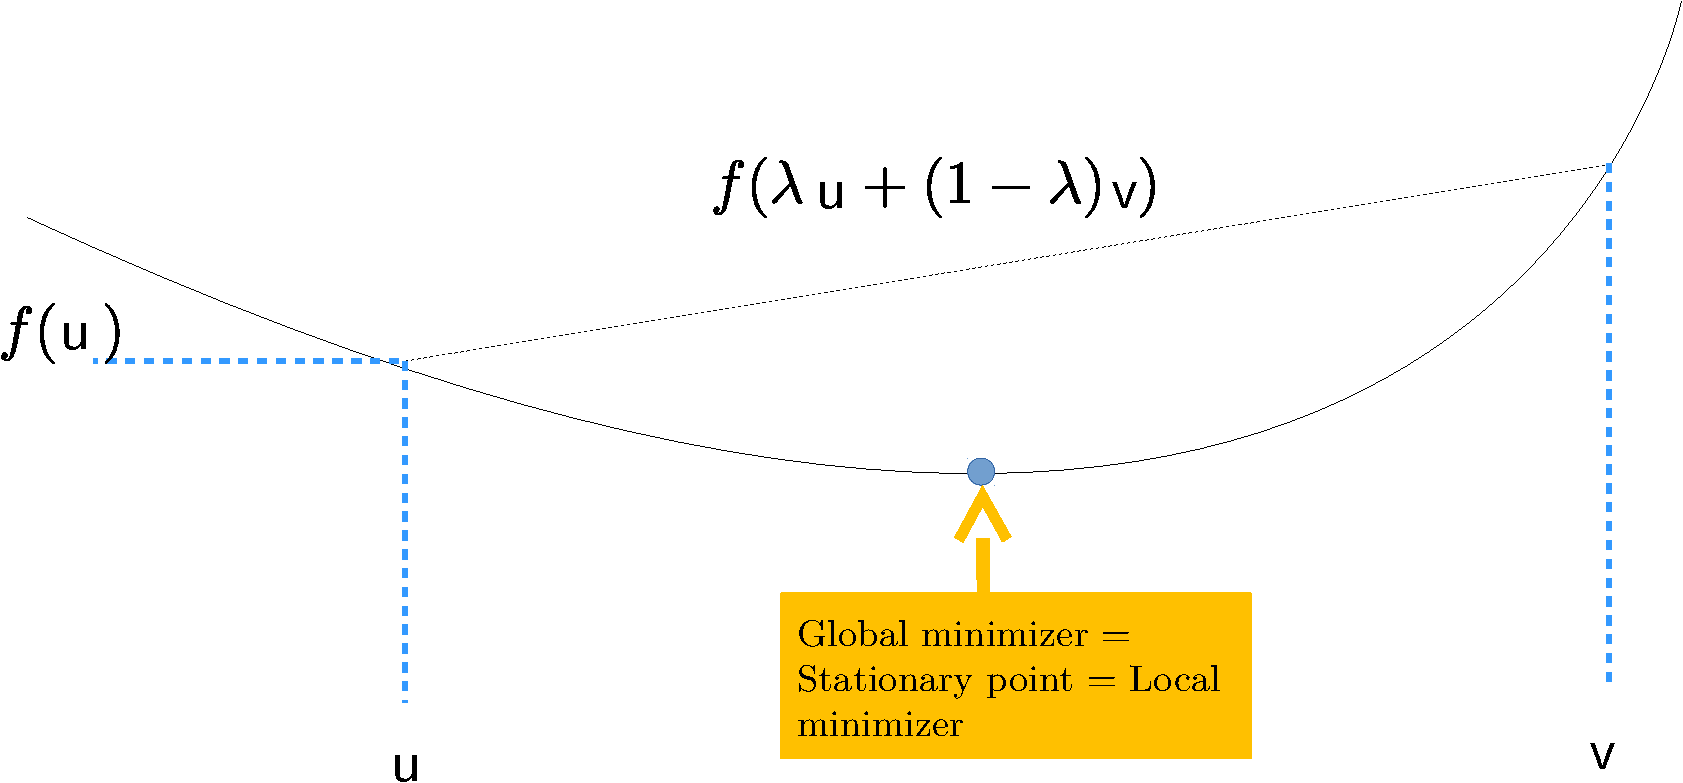
\includegraphics[width=30em]{convexity_1-crop}


\end{frame}
%%%%%%%%%%%%%%%%%%%%%%%%%%%%%%%%%%%%%%%%%%%%%%%%%%%%%%%%%%%%%%%%%%%%%%%%%%%%%%%

%%%%%%%%%%%%%%%%%%%%%%%%%%%%%%%%%%%%%%%%%%%%%%%%%%%%%%%%%%%%%%%%%%%%%%%%%%%%%%%
\begin{frame}{Convexity II}
    \begin{proposition}[Convex differentiable function]
        $f: \bbR^p \rightarrow \bbR$ is convex if and only if, $ \forall u, v \in \bbR^p$:
        \begin{align*}
            f(v)
            \geq 
            f(u) 
            + \langle \nabla f(u), v - u \rangle 
    \end{align*}
    \end{proposition}

    \centering
    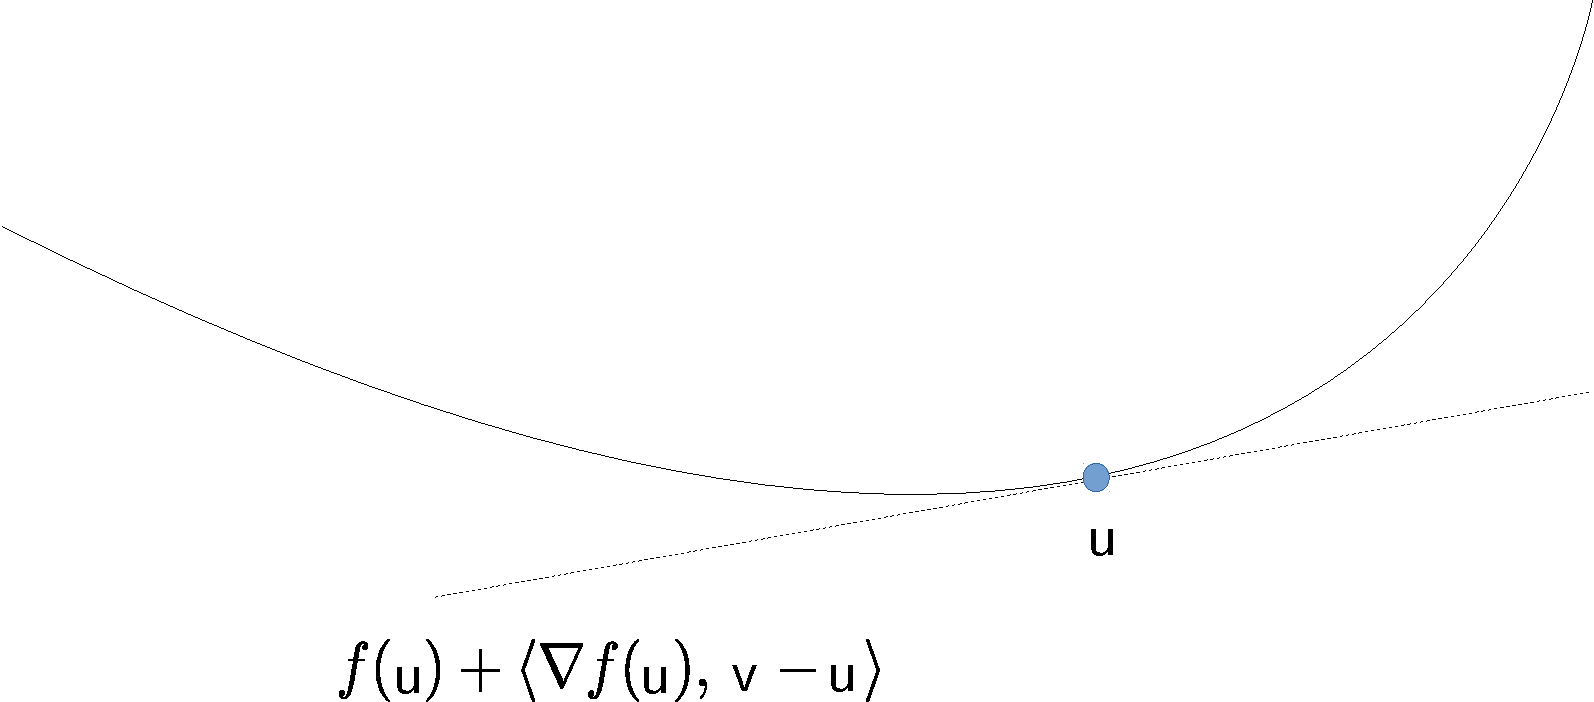
\includegraphics[width=30em]{convexity_2-crop}
    
\end{frame}
%%%%%%%%%%%%%%%%%%%%%%%%%%%%%%%%%%%%%%%%%%%%%%%%%%%%%%%%%%%%%%%%%%%%%%%%%%%%%%%

%%%%%%%%%%%%%%%%%%%%%%%%%%%%%%%%%%%%%%%%%%%%%%%%%%%%%%%%%%%%%%%%%%%%%%%%%%%%%%%
\begin{frame}{Convexity III}
    \begin{proposition}[Convex twice differentiable function]
        $f: \bbR^p \rightarrow \bbR$ is convex if and only if, $ \forall u\in \bbR^p$:
        \begin{align*}
            \nabla^2 f(u) \succeq 0
        \end{align*}
    \end{proposition}
    
    \centering
    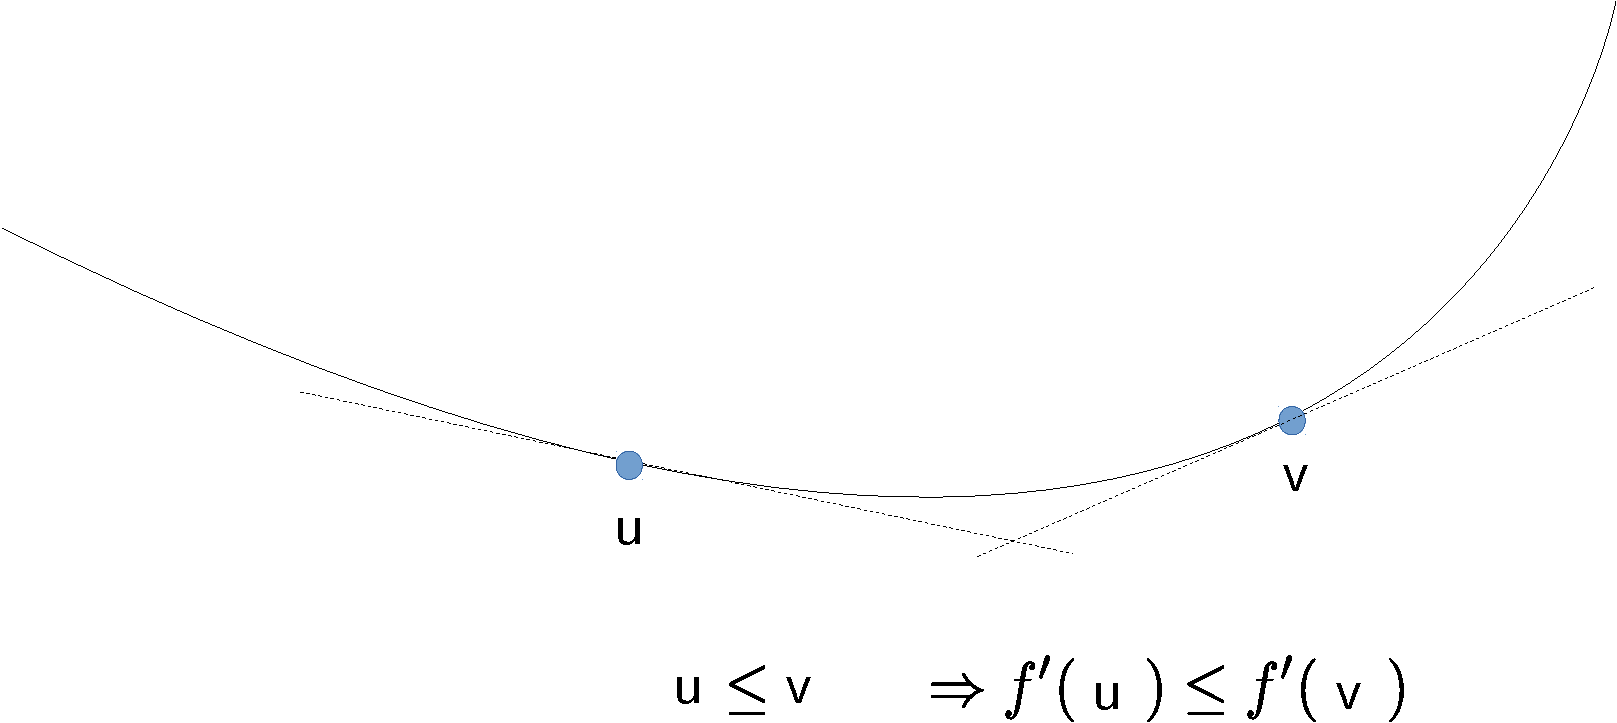
\includegraphics[width=30em]{convexity_3-crop}
\end{frame}
%%%%%%%%%%%%%%%%%%%%%%%%%%%%%%%%%%%%%%%%%%%%%%%%%%%%%%%%%%%%%%%%%%%%%%%%%%%%%%%



%%%%%%%%%%%%%%%%%%%%%%%%%%%%%%%%%%%%%%%%%%%%%%%%%%%%%%%%%%%%%%%%%%%%%%%%%%%%%%%
\begin{frame}{Strong Convexity I}
    \begin{definition}[Strongly convex function]
    $f: \bbR^p \rightarrow \bbR$ is $\mu$-strongly convex if and only if, $ \forall u, v \in \bbR^p$:
        \begin{align*}
            f(v)
            \geq 
            f(u) 
            + \langle \nabla f(u), v - u \rangle 
            + \frac{\mu}{2} \normin{v - u}^2
    \end{align*}
    \end{definition}
\end{frame}
%%%%%%%%%%%%%%%%%%%%%%%%%%%%%%%%%%%%%%%%%%%%%%%%%%%%%%%%%%%%%%%%%%%%%%%%%%%%%%%

%%%%%%%%%%%%%%%%%%%%%%%%%%%%%%%%%%%%%%%%%%%%%%%%%%%%%%%%%%%%%%%%%%%%%%%%%%%%%%%
\begin{frame}{Strong Convexity II}
    \begin{proposition}[Strongly convex twice differentiable function]
        $f: \bbR^p \rightarrow \bbR$ is $\mu$-strongly convex if and only if, $ \forall u \in \bbR^p$:
        \begin{align*}
            \nabla^2 f(u) \succeq \mu \Id_p
        \end{align*}
    \end{proposition}

\end{frame}
%%%%%%%%%%%%%%%%%%%%%%%%%%%%%%%%%%%%%%%%%%%%%%%%%%%%%%%%%%%%%%%%%%%%%%%%%%%%%%%

%%%%%%%%%%%%%%%%%%%%%%%%%%%%%%%%%%%%%%%%%%%%%%%%%%%%%%%%%%%%%%%%%%%%%%%%%%%%%%%
\begin{frame}{Smoothness}
    \begin{definition}[Smoothness]
        $f: \bbR^p \rightarrow \bbR$ is $L$-smooth if and only if, $\nabla f$ is $L$-Lipschitz
        $ \forall u, v \in \bbR^p$
        \begin{align*}
            \norm{\nabla f (u) - \nabla f (v)}
            \leq 
            L \norm{u - v}
        \end{align*}
        in particular this implies
        \begin{align*}
            f(v)
            \leq 
            f(u)
            + \langle \nabla f (u) , v - u \rangle
            + \frac{L}{2} \normin{v - u}^2
        \end{align*}
    \end{definition}
    \centering
    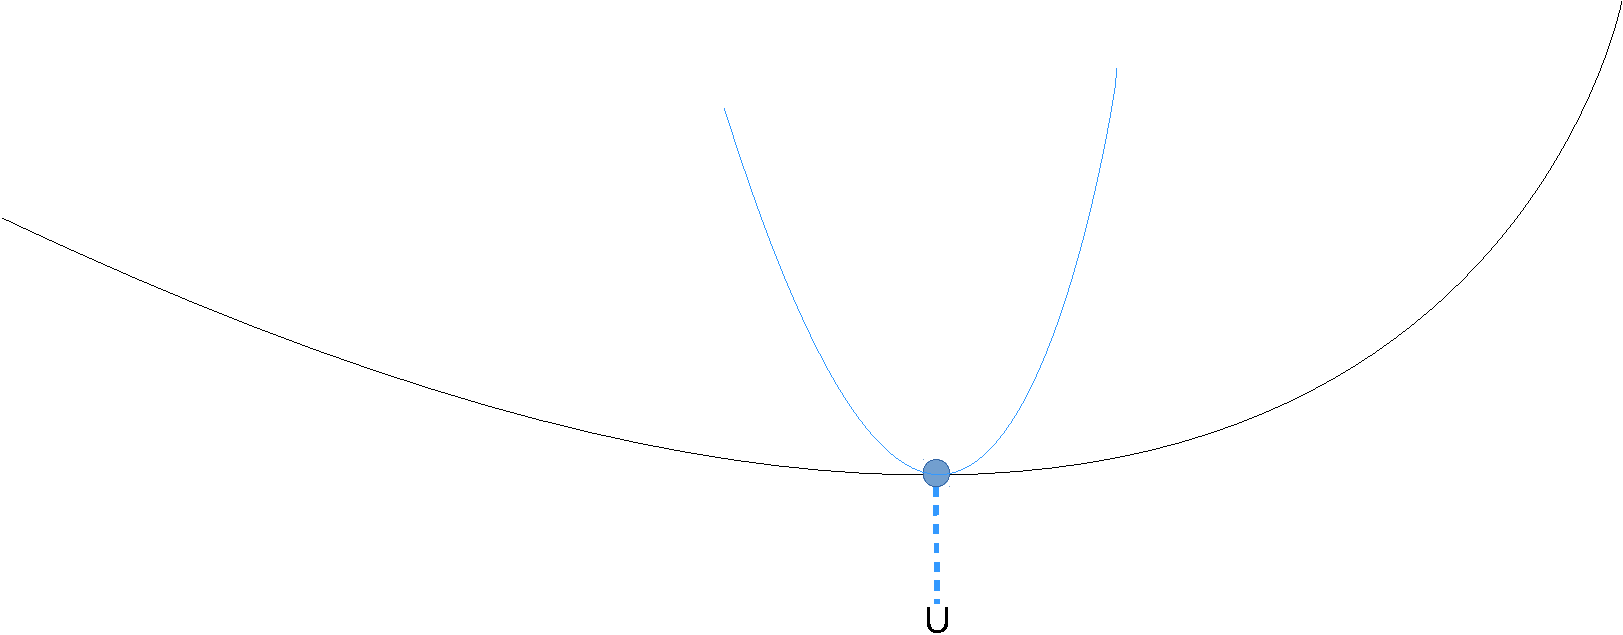
\includegraphics[width=30em]{smoothness-crop}
\end{frame}
%%%%%%%%%%%%%%%%%%%%%%%%%%%%%%%%%%%%%%%%%%%%%%%%%%%%%%%%%%%%%%%%%%%%%%%%%%%%%%%

% !TEX root = ../ds3.tex


%%%%%%%%%%%%%%%%%%%%%%%%%%%%%%%%%%%%%%%%%%%%%%%%%%%%%%%%%%%%%%%%%%%%%%%%%%%%%%%
%%%%%%%%%%%%%%%%%%%%%%%%%%%%%%%%%%%%%%%%%%%%%%%%%%%%%%%%%%%%%%%%%%%%%%%%%%%%%%%
\section{Gradient descent}
%%%%%%%%%%%%%%%%%%%%%%%%%%%%%%%%%%%%%%%%%%%%%%%%%%%%%%%%%%%%%%%%%%%%%%%%%%%%%%%
%%%%%%%%%%%%%%%%%%%%%%%%%%%%%%%%%%%%%%%%%%%%%%%%%%%%%%%%%%%%%%%%%%%%%%%%%%%%%%%


%%%%%%%%%%%%%%%%%%%%%%%%%%%%%%%%%%%%%%%%%%%%%%%%%%%%%%%%%%%%%%%%%%%%%%%%%%%%%%%
\begin{frame}{One framework to rule them all: surrogate minimization}
    \alert{Taylor expansion}
    \begin{align*}
        f(w)
        \leq
        \underbrace{f(w^{k})
        + \langle \nabla f (w^{k}), w - w^{k} \rangle
        + \frac{L}{2} \normin{w - w^{k}}^2}_{\text{Surrogate function } \tilde{f}(w)}
    \end{align*}

    \pause

    The \alert{surrogate} is minimized.
    $\tilde{f}$ is convex differentiable, infinite at the infinite (coercive), its minimum $w^*$ is achieved where gradient is 0:

    \begin{align*}
        0 = \nabla \tilde{f} (w^*) = \nabla f (w^{k}) + L (w^* - w^{k})
    \end{align*}

    \pause
    Taking $w^{k+1}$ as the minimizer of $\tilde{f}$ leads to \alert{gradient descent}:

    \begin{align*}
        w^{k+1} = w^k - \frac{1}{L} \nabla f (w^k)
    \end{align*}
\end{frame}
%%%%%%%%%%%%%%%%%%%%%%%%%%%%%%%%%%%%%%%%%%%%%%%%%%%%%%%%%%%%%%%%%%%%%%%%%%%%%%%


%%%%%%%%%%%%%%%%%%%%%%%%%%%%%%%%%%%%%%%%%%%%%%%%%%%%%%%%%%%%%%%%%%%%%%%%%%%%%%%
\begin{frame}{Example of GD}
    \centering
    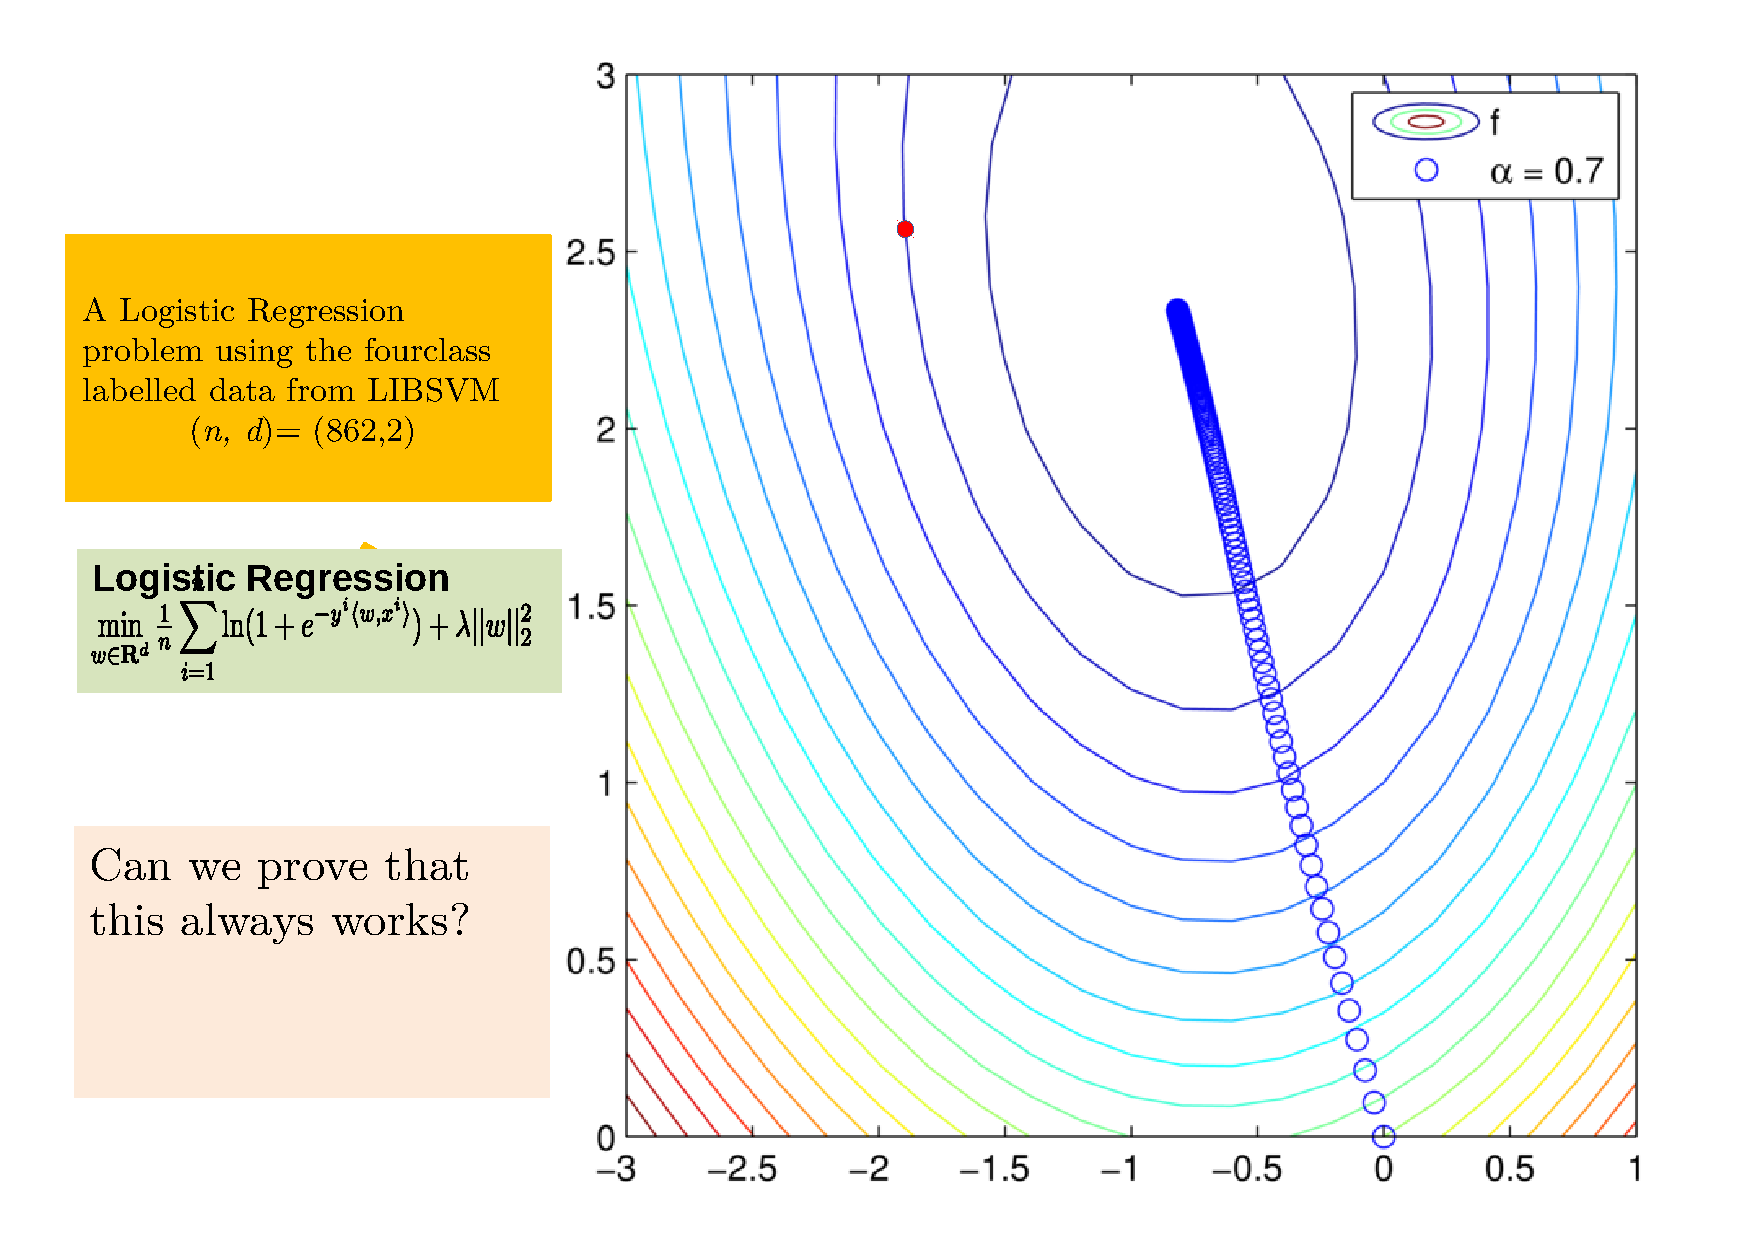
\includegraphics[width=30em]{graident_descent}

    Gradient descent on a 2D problem
\end{frame}
%%%%%%%%%%%%%%%%%%%%%%%%%%%%%%%%%%%%%%%%%%%%%%%%%%%%%%%%%%%%%%%%%%%%%%%%%%%%%%%

%%%%%%%%%%%%%%%%%%%%%%%%%%%%%%%%%%%%%%%%%%%%%%%%%%%%%%%%%%%%%%%%%%%%%%%%%%%%%%%
\begin{frame}{Line-search \footfullcite[Chap. 3]{Nocedal_Wright06}}
    What to do when a function is smooth, but you do not know the Lipschitz constant $L$? Or when $L$ is too conservative?

    \pause
    %
    Gradient descent with variable stepsize:
    %
    \begin{align*}
        w^{k+1} = w^k - \alpha^k \nabla f (w^k)
    \end{align*}
    where the stepsize $\alpha$ changes at each iteration
\end{frame}
%%%%%%%%%%%%%%%%%%%%%%%%%%%%%%%%%%%%%%%%%%%%%%%%%%%%%%%%%%%%%%%%%%%%%%%%%%%%%%%

%%%%%%%%%%%%%%%%%%%%%%%%%%%%%%%%%%%%%%%%%%%%%%%%%%%%%%%%%%%%%%%%%%%%%%%%%%%%%%%
\begin{frame}{lab0 'gradient descent line-search'}
    Your turn!

    \begin{itemize}
        \item  Play with the gradient descent to gain insight!
    \end{itemize}

\end{frame}
%%%%%%%%%%%%%%%%%%%%%%%%%%%%%%%%%%%%%%%%%%%%%%%%%%%%%%%%%%%%%%%%%%%%%%%%%%%%%%%


%%%%%%%%%%%%%%%%%%%%%%%%%%%%%%%%%%%%%%%%%%%%%%%%%%%%%%%%%%%%%%%%%%%%%%%%%%%%%%%
\begin{frame}{Gradient descent: theoretical results}
    \begin{algorithm}[H]
        \SetKwInOut{Input}{input}
        \SetKwInOut{Init}{init}
        \SetKwInOut{Parameter}{param}
        \caption{GD}
        \Init{$w^0 = 0_{p}$, $L$}
            \For{$\mathrm{iter} =1,\dots,$}
                {
                $w^{k+1} = w^k - \frac{1}{L} \nabla f (w^k)$
                }
    % \Return{$w^{}$}
    \end{algorithm}
    %
    \pause
    %
    \begin{proposition}[TODO find ref]
        If $f$ is convex and $L$-smooth, then:
        \[
        f(w^{k}) - f(w^*)
        \leq
        \frac{2 L \norm{w^0 - w^*}^2}{k}
        \]
    \end{proposition}
    %
    \pause
    %
    \begin{proposition}[TODO find ref]
        If $f$ is $\mu$-strongly convex and $L$-smooth, then:
        \[
        \normin{w^{k} - w^*}
        \leq
        \left (
            1 - \frac{\mu}{L}
        \right)^k
        \]
    \end{proposition}
\end{frame}
%%%%%%%%%%%%%%%%%%%%%%%%%%%%%%%%%%%%%%%%%%%%%%%%%%%%%%%%%%%%%%%%%%%%%%%%%%%%%%%

%%%%%%%%%%%%%%%%%%%%%%%%%%%%%%%%%%%%%%%%%%%%%%%%%%%%%%%%%%%%%%%%%%%%%%%%%%%%%%%
\begin{frame}{Exercise: lab1 'logistic gd'}
    Your turn!

    \begin{itemize}
        \item  Play with the gradient descent to gain insight!
        \item Modify the code to take into account a regularization term
    \end{itemize}

    \vspace{2em}

    Reminders!
    \begin{itemize}
        \item In all the labs the main algorithm is already coded, and we propose you to add little modifications
        \item All the solutions are in the solutions folder
    \end{itemize}
\end{frame}
%%%%%%%%%%%%%%%%%%%%%%%%%%%%%%%%%%%%%%%%%%%%%%%%%%%%%%%%%%%%%%%%%%%%%%%%%%%%%%%

% !TEX root = ../ds3.tex

%%%%%%%%%%%%%%%%%%%%%%%%%%%%%%%%%%%%%%%%%%%%%%%%%%%%%%%%%%%%%%%%%%%%%%%%%%%%%%%
%%%%%%%%%%%%%%%%%%%%%%%%%%%%%%%%%%%%%%%%%%%%%%%%%%%%%%%%%%%%%%%%%%%%%%%%%%%%%%%
\section{Newton method}
%%%%%%%%%%%%%%%%%%%%%%%%%%%%%%%%%%%%%%%%%%%%%%%%%%%%%%%%%%%%%%%%%%%%%%%%%%%%%%%
%%%%%%%%%%%%%%%%%%%%%%%%%%%%%%%%%%%%%%%%%%%%%%%%%%%%%%%%%%%%%%%%%%%%%%%%%%%%%%%


%%%%%%%%%%%%%%%%%%%%%%%%%%%%%%%%%%%%%%%%%%%%%%%%%%%%%%%%%%%%%%%%%%%%%%%%%%%%%%%
\begin{frame}{Newton method: intuition}
%
\alert{Taylor expansion} to the order 2:
%
    \begin{align*}
        f(w^{k+1}) 
        \sim &
        f(w^{k}) 
        + \langle \nabla f (w^{k}), w^{k+1} - w^{k} \rangle 
        \\
        &\underbrace{+ \frac{1}{2} (w^{k+1} - w^{k})^\top \nabla^2 f (w^{k}) (w^{k+1} - w^{k})}_{\tilde{f}(w^{k+1})}
    \end{align*}
%
\pause
%
The \alert{`surrogate`} is minimized:
    \begin{align*}
        0 
        & = \nabla \tilde{f}(w^{k+1})
        = \nabla f (w^{k})
        + \nabla^2 f (w^{k}) (w^{k+1} - w^{k})
    \end{align*}
%
\pause
%
This leads to the following update for the \alert{Newton algorithm}:
    \begin{align*}
        w^{k+1} 
        &= 
        w^{k} 
        - [\nabla^2 f (w^{k})]^{-1} \nabla f (w^{k})
    \end{align*}
%
\pause
%
\center
What about convergence guarantees?
\end{frame}
%%%%%%%%%%%%%%%%%%%%%%%%%%%%%%%%%%%%%%%%%%%%%%%%%%%%%%%%%%%%%%%%%%%%%%%%%%%%%%%


%%%%%%%%%%%%%%%%%%%%%%%%%%%%%%%%%%%%%%%%%%%%%%%%%%%%%%%%%%%%%%%%%%%%%%%%%%%%%%%
\begin{frame}[t]\frametitle{Convergence of Newton method}
    \begin{Theorem}[Convergence of Newton method]
    Suppose that $f$ is twice differentiable, and the Hessian $\nabla^2 f(w^*)$ is Lipschitz continuous in a neighborhood of a solution $w^*$
    such that $\nabla f(w^*) = 0$ and $\nabla^2 f(w^*) \succ 0$.
    
    Then there exists a closed ball $\mathcal{B}$ centered on $w^*$,
    such that for every $w^0 \in \mathcal{B}$, the sequence $w^k$ obtained
    with Newton algorithm stays in $\mathcal{B}$ and converges towards $w^*$.
    Furthermore, there is a constant $\gamma > 0$, such that
    $\|w^{k+1} - w^* \| \leq \gamma \|w^{k} - w^* \|^2$.
    \end{Theorem}
    \pause
    Drawbacks:
    \begin{itemize}
        \item \alert{Convergence} of Newton is \alert{local} (see proof in \footfullcite[Thm. 3.5]{Nocedal_Wright06}).
        The method \alert{may diverge} if the initial point is too far
        from $w^*$ or if the Hessian is \alert{not positive definite}
        \item One has to solve a linear system at each step! $O(p^3)$
    \end{itemize}
\end{frame}
%%%%%%%%%%%%%%%%%%%%%%%%%%%%%%%%%%%%%%%%%%%%%%%%%%%%%%%%%%%%%%%%%%%%%%%%%%%%%%%

%%%%%%%%%%%%%%%%%%%%%%%%%%%%%%%%%%%%%%%%%%%%%%%%%%%%%%%%%%%%%%%%%%%%%%%%%%%%%%%
\begin{frame}[t]\frametitle{From Newton to quasi-Newton}
    %
    
    Idea:
    \begin{itemize}
        \item Construct iterative approximations of the inverse of the Hessian \footfullcite{Nocedal1980}
        \item Combine it with line-search strategies
    \end{itemize}
    
    \pause
    \vspace{1em} 

    \begin{equation*}
        \begin{cases}
            d^k 
            &= -B^k g^k 
            \quad \text{find a \alert{descent direction}}
            \\
            w^{k+1} 
            &= w^k + \alpha^k d^k
             \quad \text{\alert{line-search}}
        \end{cases}
    \end{equation*}
    
    \vspace{2em}
    
    \textcolor{blue}{TODO finish talk about multiples update rules}
    
\end{frame}
%%%%%%%%%%%%%%%%%%%%%%%%%%%%%%%%%%%%%%%%%%%%%%%%%%%%%%%%%%%%%%%%%%%%%%%%%%%%%%%

%%%%%%%%%%%%%%%%%%%%%%%%%%%%%%%%%%%%%%%%%%%%%%%%%%%%%%%%%%%%%%%%%%%%%%%%%%%%%%%
\begin{frame}{Exercise: lab2 'logistic Newton'}
    Your turn!
    
    \begin{itemize}
        \item  Play with L-BFGS to gain insight! 
        \item Implement an $\ell_2$ regularized logistic regression with bias yourself!
        \item Implement a Newton method yourself!
    \end{itemize}
    
    \vspace{2em}
    
    Reminders! 
    \begin{itemize}
        \item In all the labs the main algorithm is already coded, and we propose you to add little modifications
        \item All the solutions are in the solutions folder
    \end{itemize}
\end{frame}
%%%%%%%%%%%%%%%%%%%%%%%%%%%%%%%%%%%%%%%%%%%%%%%%%%%%%%%%%%%%%%%%%%%%%%%%%%%%%%%

% !TEX root = ../ds3.tex

%%%%%%%%%%%%%%%%%%%%%%%%%%%%%%%%%%%%%%%%%%%%%%%%%%%%%%%%%%%%%%%%%%%%%%%%%%%%%%%
%%%%%%%%%%%%%%%%%%%%%%%%%%%%%%%%%%%%%%%%%%%%%%%%%%%%%%%%%%%%%%%%%%%%%%%%%%%%%%%
\section{Stochastic gradient descent}
%%%%%%%%%%%%%%%%%%%%%%%%%%%%%%%%%%%%%%%%%%%%%%%%%%%%%%%%%%%%%%%%%%%%%%%%%%%%%%%
%%%%%%%%%%%%%%%%%%%%%%%%%%%%%%%%%%%%%%%%%%%%%%%%%%%%%%%%%%%%%%%%%%%%%%%%%%%%%%%


%%%%%%%%%%%%%%%%%%%%%%%%%%%%%%%%%%%%%%%%%%%%%%%%%%%%%%%%%%%%%%%%%%%%%%%%%%%%%%%
\begin{frame}{Optimization for ML: finite sum}
    Optimization in general:
    %
    \begin{align*}
        \min_{x \in \bbR^p} f(x)
    \end{align*}

    \pause

    Optimization for Machine Learning:
    %
    \begin{align*}
        \min_{x \in \bbR^p} f(x) \eqdef \sum_i^n f_i(x)
    \end{align*}

    \pause

    \begin{itemize}
        \item Can we take advantage of this \alert{finite sum} structure?
        \item In particular when the number of samples $n$ is large?
    \end{itemize}

\end{frame}
%%%%%%%%%%%%%%%%%%%%%%%%%%%%%%%%%%%%%%%%%%%%%%%%%%%%%%%%%%%%%%%%%%%%%%%%%%%%%%%

%%%%%%%%%%%%%%%%%%%%%%%%%%%%%%%%%%%%%%%%%%%%%%%%%%%%%%%%%%%%%%%%%%%%%%%%%%%%%%%
\begin{frame}{Stochastic Gradient Descent (SGD)}
    %
    \begin{itemize}
        \item Full gradient methods can be expensive
        \item \alert{Idea:} use a \alert{single gradient} $\nabla f_i(w)$ \alert{instead of of full gradient} $\sum_i^n \nabla f_i (w)$
    \end{itemize}
    %
    \vspace{2em}
    %
\begin{minipage}{0.49 \textwidth}
    \begin{algorithm}[H]
        \SetKwInOut{Input}{input}
        \SetKwInOut{Init}{init}
        \SetKwInOut{Parameter}{param}
        \caption{SGD}
        \Init{ $w = 0_{p}$, $\alpha$}
            \For{$\mathrm{iter} =1,\dots,$}
                {
                Sample $i$ in $1, \dots, n$

                \tcp{Single gradient $\nabla f_i(w)$ call}

                $w \leftarrow w - \alpha \nabla f_i (w)$

                }
    \Return{$w$}
    \end{algorithm}
\end{minipage}
%
\begin{minipage}{0.49 \textwidth}
    \begin{algorithm}[H]
        \SetKwInOut{Input}{input}
        \SetKwInOut{Init}{init}
        \SetKwInOut{Parameter}{param}
        \caption{GD}
        \Init{ $w = 0_{p}$, $\alpha$}
            \For{$\mathrm{iter} =1,\dots,$}
                {
                    \tcp{Full gradient $\nabla f (w)$ call}

                    $w \leftarrow w - \alpha \nabla f (w)$
                }
    \Return{$w$}
    \end{algorithm}
\end{minipage}
\end{frame}
%%%%%%%%%%%%%%%%%%%%%%%%%%%%%%%%%%%%%%%%%%%%%%%%%%%%%%%%%%%%%%%%%%%%%%%%%%%%%%%

%%%%%%%%%%%%%%%%%%%%%%%%%%%%%%%%%%%%%%%%%%%%%%%%%%%%%%%%%%%%%%%%%%%%%%%%%%%%%%%
\begin{frame}{SGD wit constant stepsize $\alpha$: theoretical results}
    \begin{proposition}[TODO find ref]
        If $f$ is $\mu$-strongly convex and $L$-smooth, then:
        \[
        \bbE ( \normin{w^{k} - w^*}^2 )
        \leq
        \left (
            1 - \alpha \mu
        \right)^k
        \normin{w^0 - w^*}^2
        +
        \frac{\alpha}{\mu} C
        \enspace .
        \]
    \end{proposition}
    %
    \begin{center}
        \alert{
            SGD with constant stepsize does not converge}
    \end{center}

\end{frame}
%%%%%%%%%%%%%%%%%%%%%%%%%%%%%%%%%%%%%%%%%%%%%%%%%%%%%%%%%%%%%%%%%%%%%%%%%%%%%%%

%%%%%%%%%%%%%%%%%%%%%%%%%%%%%%%%%%%%%%%%%%%%%%%%%%%%%%%%%%%%%%%%%%%%%%%%%%%%%%%
\begin{frame}{Example of SGD}
    \centering
    \only<1>{
        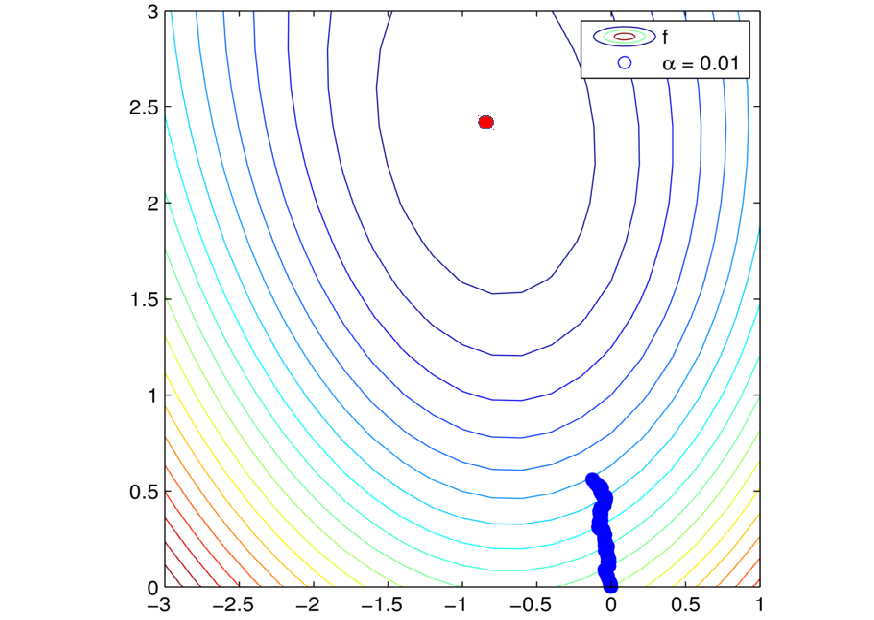
\includegraphics[width=30em]{sgd_1}
    }%
    \only<2>{
        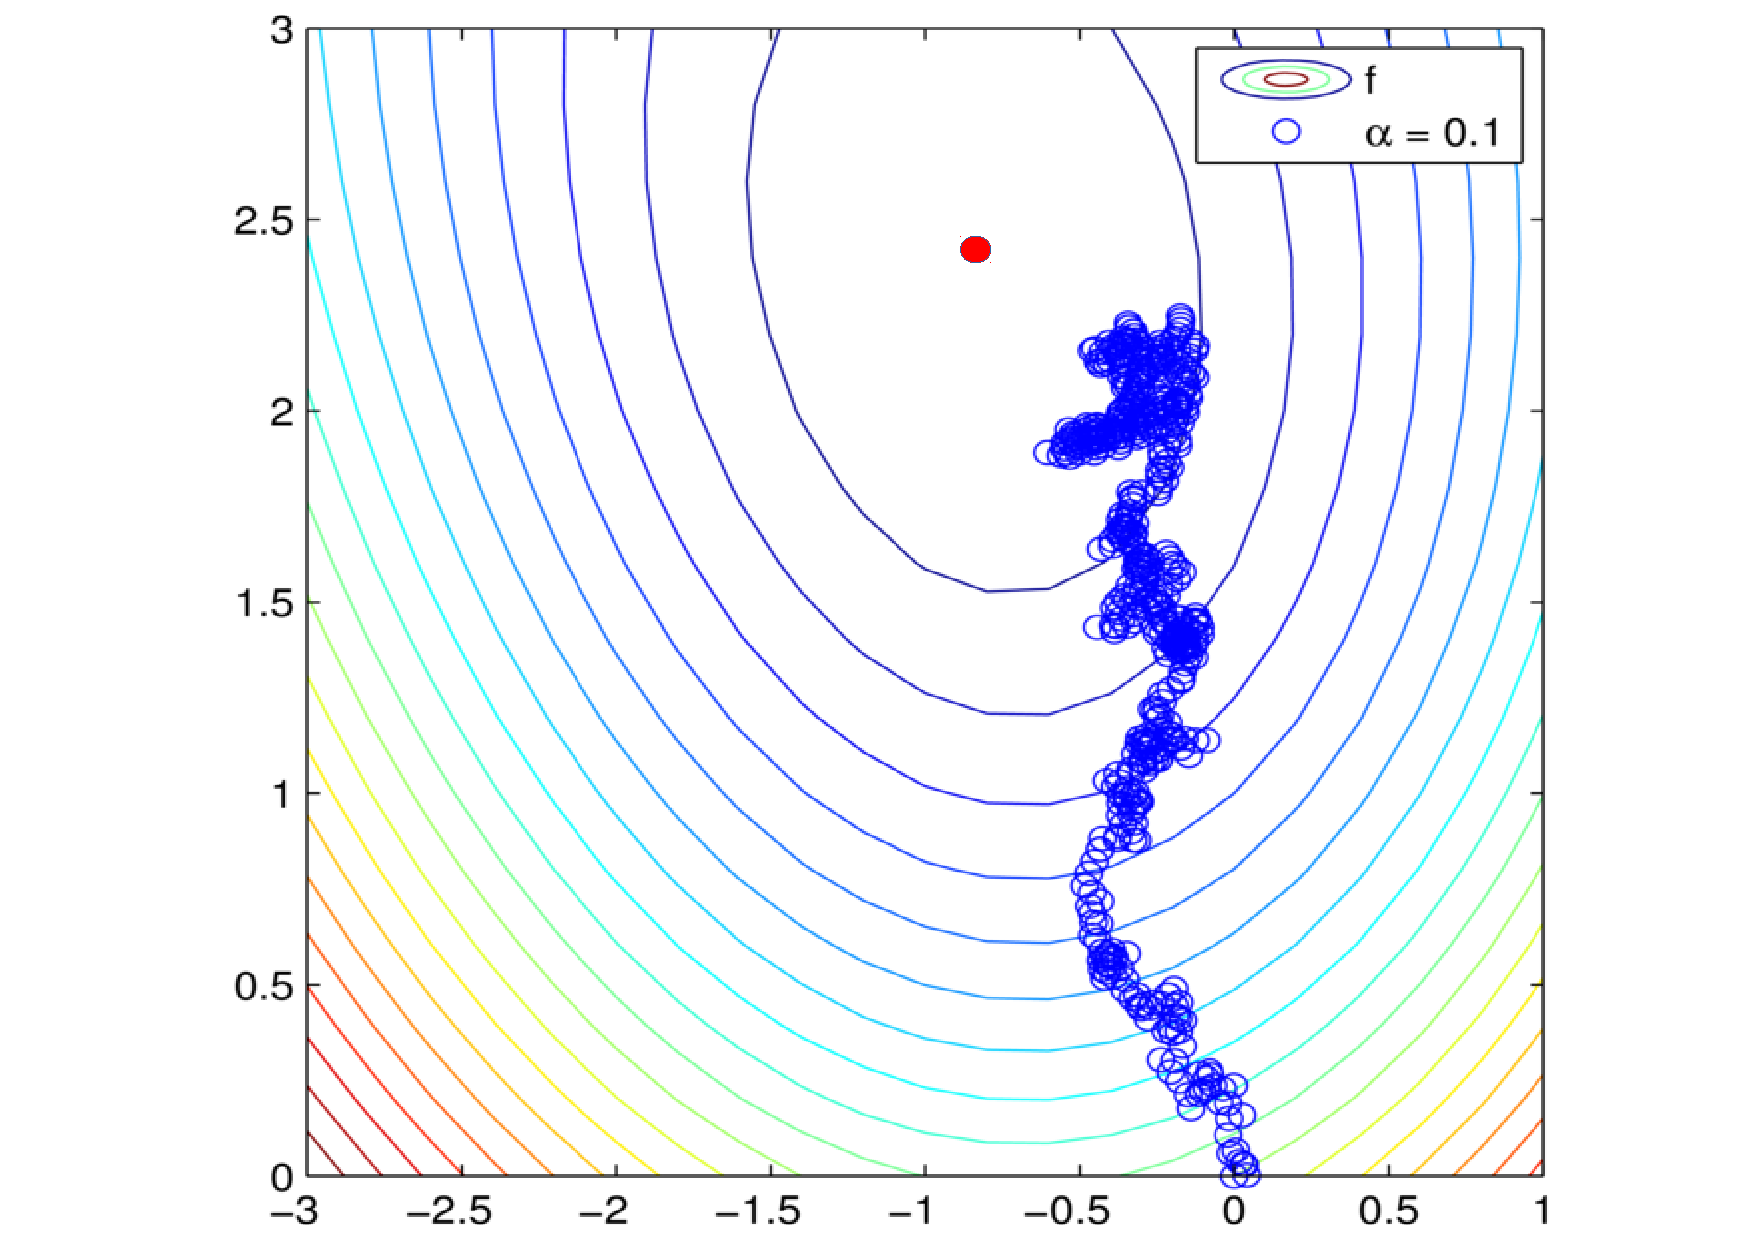
\includegraphics[width=30em]{sgd_2}
    }%
    \only<3>{
        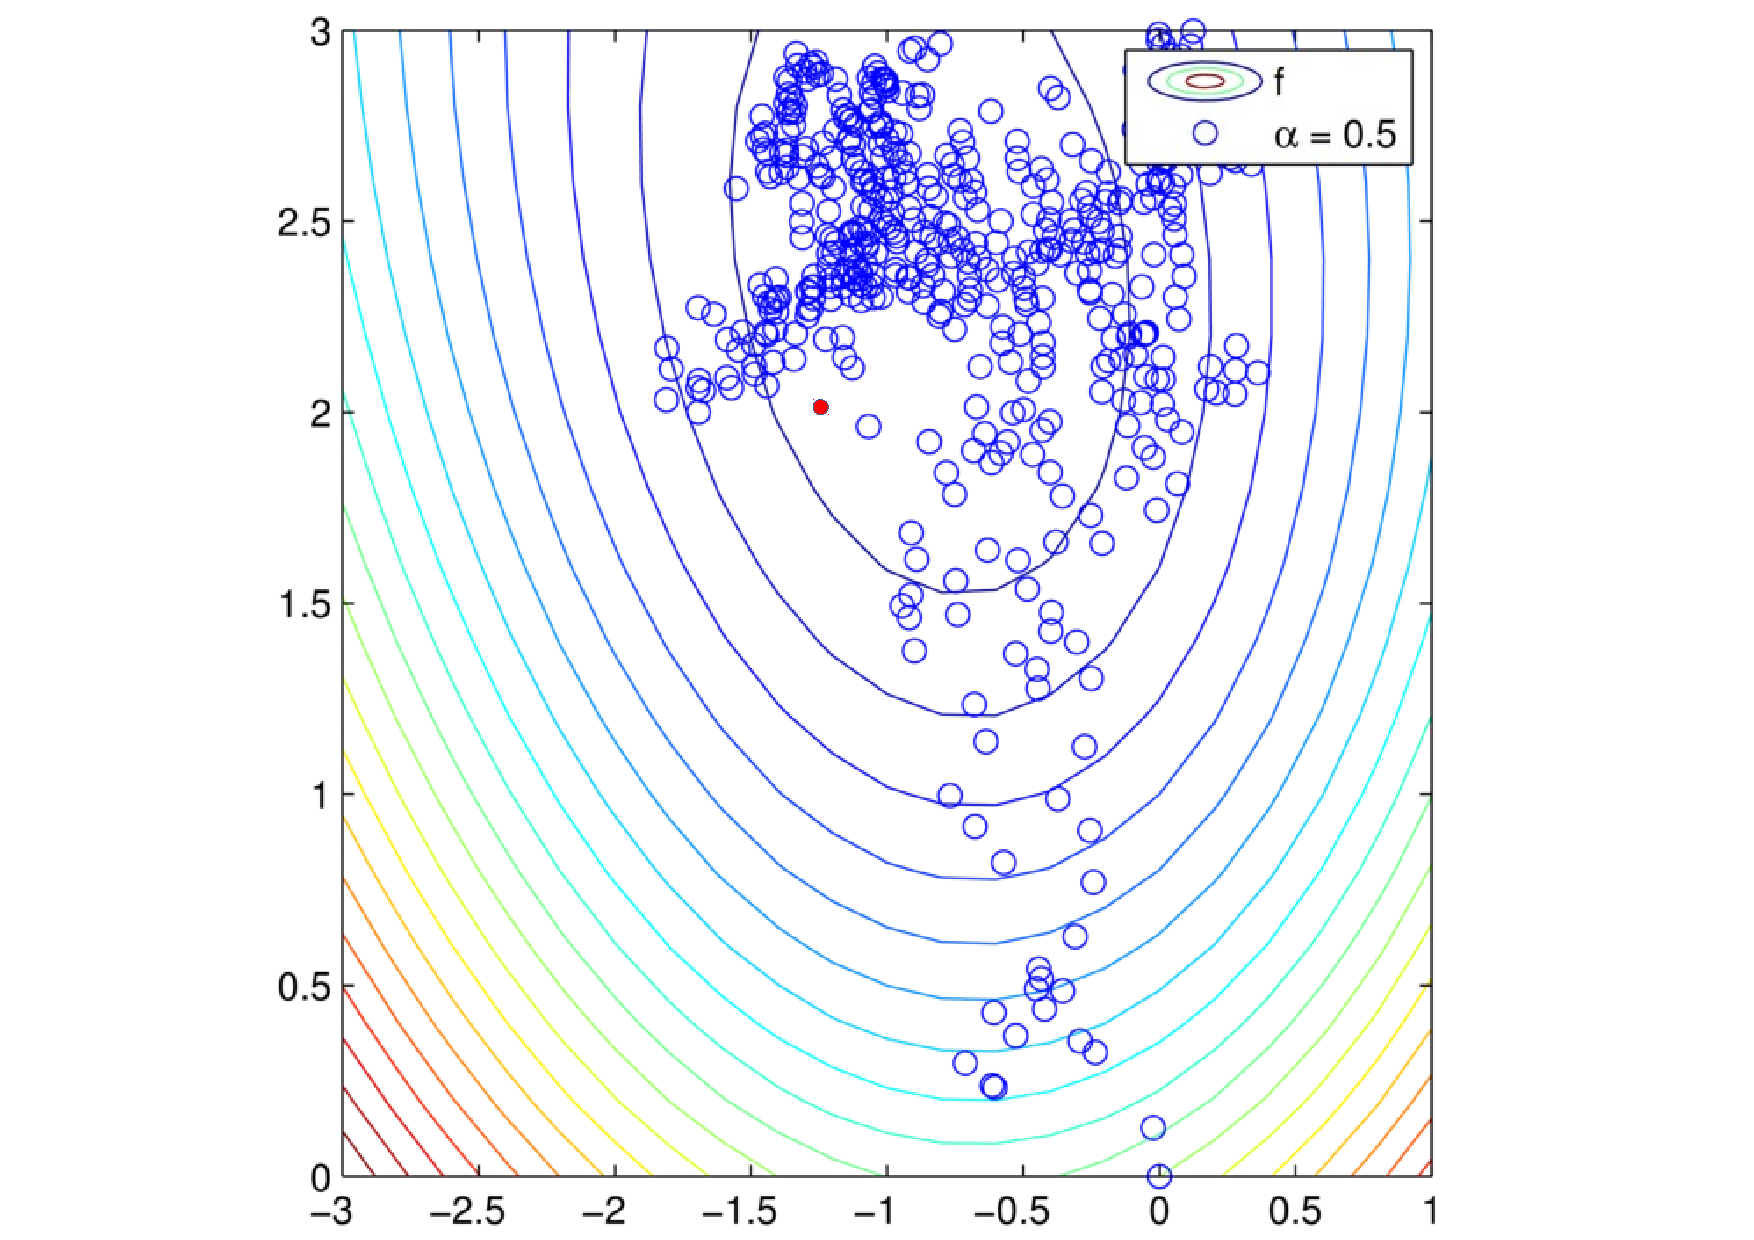
\includegraphics[width=30em]{sgd_3}
    }
    SGD on a 2D problem
\end{frame}
%%%%%%%%%%%%%%%%%%%%%%%%%%%%%%%%%%%%%%%%%%%%%%%%%%%%%%%%%%%%%%%%%%%%%%%%%%%%%%%

%%%%%%%%%%%%%%%%%%%%%%%%%%%%%%%%%%%%%%%%%%%%%%%%%%%%%%%%%%%%%%%%%%%%%%%%%%%%%%%
\begin{frame}{Exercise: lab3 'stochastic gradient descent'}
    Your turn!

    \begin{itemize}
        \item  Play with SGD to gain insight: make $n$ vary!
        \item Play with the regularization parameter $\lambda$
        \item Play with the correlation of the data to see what's happening
    \end{itemize}

    \vspace{2em}

    Reminders!
    \begin{itemize}
        \item In all the labs the main algorithm is already coded, and we propose you to add little modifications
        \item All the solutions are in the solutions folder
    \end{itemize}
\end{frame}
%%%%%%%%%%%%%%%%%%%%%%%%%%%%%%%%%%%%%%%%%%%%%%%%%%%%%%%%%%%%%%%%%%%%%%%%%%%%%%%

% !TEX root = ../ds3.tex

%%%%%%%%%%%%%%%%%%%%%%%%%%%%%%%%%%%%%%%%%%%%%%%%%%%%%%%%%%%%%%%%%%%%%%%%%%%%%%%
%%%%%%%%%%%%%%%%%%%%%%%%%%%%%%%%%%%%%%%%%%%%%%%%%%%%%%%%%%%%%%%%%%%%%%%%%%%%%%%
\section{Coordinate descent}
%%%%%%%%%%%%%%%%%%%%%%%%%%%%%%%%%%%%%%%%%%%%%%%%%%%%%%%%%%%%%%%%%%%%%%%%%%%%%%%
%%%%%%%%%%%%%%%%%%%%%%%%%%%%%%%%%%%%%%%%%%%%%%%%%%%%%%%%%%%%%%%%%%%%%%%%%%%%%%%


%%%%%%%%%%%%%%%%%%%%%%%%%%%%%%%%%%%%%%%%%%%%%%%%%%%%%%%%%%%%%%%%%%%%%%%%%%%%%%%
\begin{frame}{Exact Coordinate Descent: idea}

    Goal:
    \begin{align*}
        \min_{w \in \mathbb{R}^p} f(w_1, \dots, w_p)
    \end{align*}
    %
    \pause
    %
    Idea: solve \alert{smaller} and \alert{simpler subproblems}
    %
    \pause

    Algorithm:
    \begin{equation*}
        \begin{aligned}
        \text{for iter}
            & = 1, \dots
            \\
            \text{for }
            & j = 1, \dots, p \quad \text{(cyclic rule)}
            \\
                &
                w_{j}
                \leftarrow
                \argmin_{z \in \mathbb{R}}
                f(w_1, \ldots, w_{j-1}, z, w_{j+1}, \ldots, w_p)
         \end{aligned}
    \end{equation*}
    %
    \pause
    %
    Remarks
    \begin{itemize}
        \item The order of cycle through coordinates is arbitrary, can use any
    permutation of ${1, 2, \dots, n}$
        \item We just have to solve 1D optimization problems but a lot of them...
    \end{itemize}
\end{frame}
%%%%%%%%%%%%%%%%%%%%%%%%%%%%%%%%%%%%%%%%%%%%%%%%%%%%%%%%%%%%%%%%%%%%%%%%%%%%%%%

%%%%%%%%%%%%%%%%%%%%%%%%%%%%%%%%%%%%%%%%%%%%%%%%%%%%%%%%%%%%%%%%%%%%%%%%%%%%%%%
\begin{frame}{Example of CD}
    \centering
    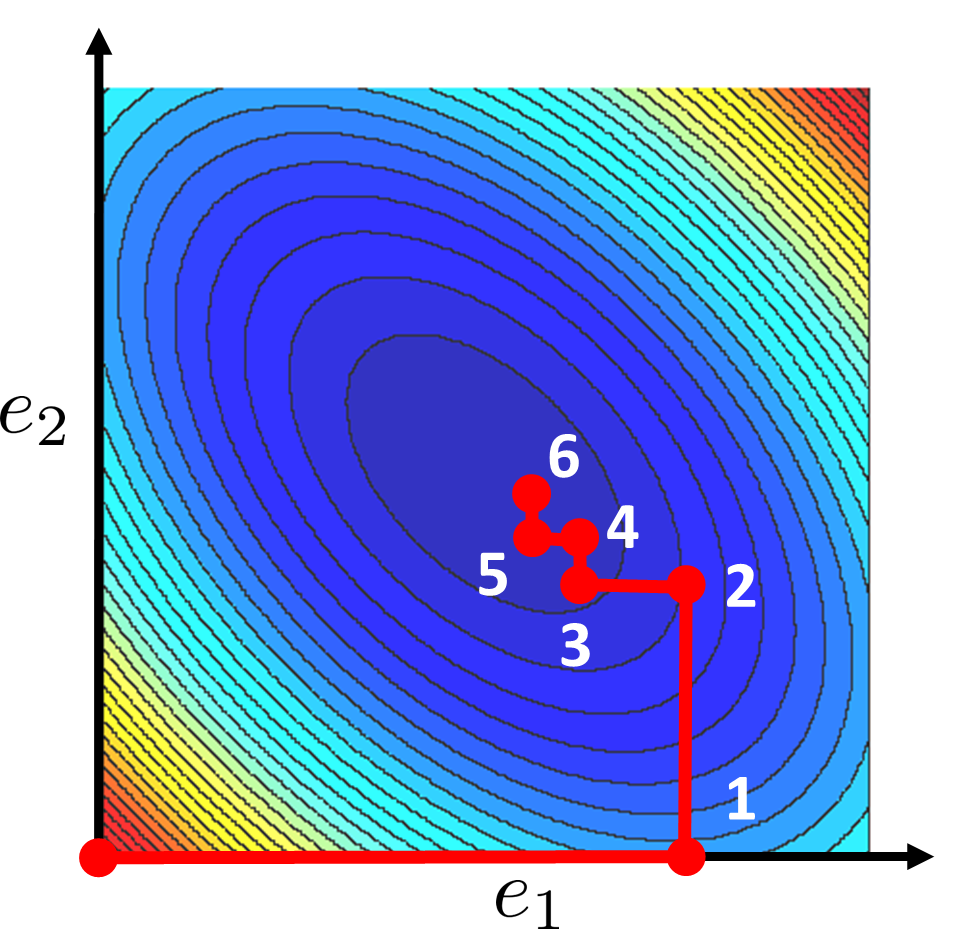
\includegraphics[width=17em]{exampleCD}

    Coordinate descent on a 2D problem
\end{frame}
%%%%%%%%%%%%%%%%%%%%%%%%%%%%%%%%%%%%%%%%%%%%%%%%%%%%%%%%%%%%%%%%%%%%%%%%%%%%%%%

%%%%%%%%%%%%%%%%%%%%%%%%%%%%%%%%%%%%%%%%%%%%%%%%%%%%%%%%%%%%%%%%%%%%%%%%%%%%%%%
\begin{frame}{Exercise: linear regression}
    Derive the exact coordinate descent algorithm for
    \begin{align*}
        f(x)= \frac{1}{2} \|y - A x\|^2
        \enspace ,
    \end{align*}
    where $y \in \bbR^p$, $A \in \bbR^{n \times p}$ is the design matrix.

    \medskip
    \pause

    \textcolor{blue}{TODO correction}

\end{frame}
%%%%%%%%%%%%%%%%%%%%%%%%%%%%%%%%%%%%%%%%%%%%%%%%%%%%%%%%%%%%%%%%%%%%%%%%%%%%%%%

%%%%%%%%%%%%%%%%%%%%%%%%%%%%%%%%%%%%%%%%%%%%%%%%%%%%%%%%%%%%%%%%%%%%%%%%%%%%%%%
\begin{frame}{Coordinate Gradient Descent: algorithm}
    %
    \begin{itemize}
        \item Exact minimization can be expensive
        \item \alert{Idea:} do a \alert{local gradient step} instead of exact minimization
    \end{itemize}
\begin{minipage}{0.49 \textwidth}
    \begin{algorithm}[H]
        \SetKwInOut{Input}{input}
        \SetKwInOut{Init}{init}
        \SetKwInOut{Parameter}{param}
        \caption{CD}
        \Init{ $w = 0_{p}$, $L_1$, \dots, $L_p$}
            \For{$\mathrm{iter} =1,\dots,$}
                {
                \For{$j = 1, \dots, p$}
                    {
                    \tcp{Update only one coef.}

                    $w_j \leftarrow w_j - \frac{1}{L_j} \nabla_j f (w)$
                    }
                }
    \Return{$w$}
    \end{algorithm}
\end{minipage}
%
\begin{minipage}{0.49 \textwidth}
    \begin{algorithm}[H]
        \SetKwInOut{Input}{input}
        \SetKwInOut{Init}{init}
        \SetKwInOut{Parameter}{param}
        \caption{GD}
        \Init{ $w = 0_{p}$, $L$}
            \For{$\mathrm{iter} =1,\dots,$}
                {
                    \tcp{Update all the coef.}

                    $w \leftarrow w - \frac{1}{L} \nabla f (w)$
                }
    \Return{$w$}
    \end{algorithm}
\end{minipage}
\end{frame}
%%%%%%%%%%%%%%%%%%%%%%%%%%%%%%%%%%%%%%%%%%%%%%%%%%%%%%%%%%%%%%%%%%%%%%%%%%%%%%%

%%%%%%%%%%%%%%%%%%%%%%%%%%%%%%%%%%%%%%%%%%%%%%%%%%%%%%%%%%%%%%%%%%%%%%%%%%%%%%%
\begin{frame}{Convergence speed of CD \footfullcite{Beck_Tetruashvili13}}
    Assume $f$ is convex; $\nabla f$ is Lipschitz continuous; $\gamma_j = \frac{1}{L_j}$
    \begin{proposition}[Beck and Tetruashvili (2013)]
    \[
    f(w^{k+1}) - f(w^*)
    \leq
    4 L_{\max} (1+n^3 L_{\max}^2 / L_{\min}^2 ) \frac{R^2(w^0)}{k + 8/n}
    \]
    where
    $R^2(w^0)
    =
    \max_{u, v \in \cV} \{ \|u - v\| :
    f(v) \leq f(u) \leq f(w^0)\}$,
    $L_{\max} = \max_i L_i$
    and $L_{\min} = \min_i L_i$.
    \end{proposition}

    \begin{itemize}
        \item \alert{worst} case complexity rates of CD are bad ($n^3$ complexity) because it is possible to construct adversarial examples \footfullcite{Sun_Ye2019}
        \item However \alert{CD performs surprisingly well} on real-world problems (see labs)
    \end{itemize}
\end{frame}
%%%%%%%%%%%%%%%%%%%%%%%%%%%%%%%%%%%%%%%%%%%%%%%%%%%%%%%%%%%%%%%%%%%%%%%%%%%%%%%


%%%%%%%%%%%%%%%%%%%%%%%%%%%%%%%%%%%%%%%%%%%%%%%%%%%%%%%%%%%%%%%%%%%%%%%%%%%%%%%
\begin{frame}{Exercise: lab4}
    Your turn! Code an $\ell_2$ regularized logistic regression with bias

    \vspace{2em}

    Reminder! All the solutions are in the solutions folder
\end{frame}
%%%%%%%%%%%%%%%%%%%%%%%%%%%%%%%%%%%%%%%%%%%%%%%%%%%%%%%%%%%%%%%%%%%%%%%%%%%%%%%

% !TEX root = ../ds3.tex

%%%%%%%%%%%%%%%%%%%%%%%%%%%%%%%%%%%%%%%%%%%%%%%%%%%%%%%%%%%%%%%%%%%%%%%%%%%%%%%
%%%%%%%%%%%%%%%%%%%%%%%%%%%%%%%%%%%%%%%%%%%%%%%%%%%%%%%%%%%%%%%%%%%%%%%%%%%%%%%
\section{Nonsmooth optimization}
%%%%%%%%%%%%%%%%%%%%%%%%%%%%%%%%%%%%%%%%%%%%%%%%%%%%%%%%%%%%%%%%%%%%%%%%%%%%%%%
%%%%%%%%%%%%%%%%%%%%%%%%%%%%%%%%%%%%%%%%%%%%%%%%%%%%%%%%%%%%%%%%%%%%%%%%%%%%%%%


%%%%%%%%%%%%%%%%%%%%%%%%%%%%%%%%%%%%%%%%%%%%%%%%%%%%%%%%%%%%%%%%%%%%%%%%%%%%%%%
\begin{frame}{Nonsmooth optimization}
    \textcolor{blue}{TODO if time}
\end{frame}
%%%%%%%%%%%%%%%%%%%%%%%%%%%%%%%%%%%%%%%%%%%%%%%%%%%%%%%%%%%%%%%%%%%%%%%%%%%%%%%



%%%%%%%%%%%%%%%%%%%%%%%%%%%%%%%%%%%%%%%%%%%%%%%%%%%%%%%%%%%%%%%%%%%%%%%%%%%%%%%
\begin{frame}[allowframebreaks]
   \printbibliography
\end{frame}
%%%%%%%%%%%%%%%%%%%%%%%%%%%%%%%%%%%%%%%%%%%%%%%%%%%%%%%%%%%%%%%%%%%%%%%%%%%%%%%



\end{document}
